\documentclass{article}

\usepackage[margin=1in]{geometry} % Set margins to 1 inch
\usepackage{graphicx} % Allows including images
\usepackage{float} % Allows for precise placement of figures
\usepackage{amsmath} % Allows for math equations
\usepackage{siunitx} % Allows for SI units
\usepackage{placeins} % Makes sure images are in their respective sections by \FloatBarrier

\begin{document}

\title{Hardware Assignment Report\\ \large{Aditya Gawande\\EE22BTECH11202}}
\author{}
\date{}
\maketitle

\maketitle

\section*{Description}

\subsection*{Setup}
\begin{itemize}
    \item This circuit uses 5V from microusb.
    \item This acts as the Vcc of the circuit. 
    \item The inner buses on both sides are at Vcc. 
    \item The lowest bus is GND. 
    \item The uppermost bus is carrying the Clock signal from the 555 timer.
\end{itemize}

\subsection*{Circuit Overview}
\begin{enumerate}
    \item The Flipflops take clock from the clock bus and based on their initial state, output a sequence of numbers.
    \item The sequence is fixed and if the circuit is operated without concern for the initial state, the output number shown is generated randomly from 1 to 15 (both inclusive), with equal probability of all of them.
    \item The decoder is able to show numbers from 0 to 15, and the ABCD formed by the flipflops do not become 0000 at any point of time.
    \item The output repeats after all 16 numbers are shown.
    \item This circuit is deterministic, hence, the randomness can be decoded out by simply refering to the sequence. 
    \item Sequence generated by this sequence is 3,7,15,14,13,10,5,11,6,12,9,2,4,8,1,3,7.....
\end{enumerate}
\subsubsection*{Timer}
\begin{enumerate}
    \item The time period can be changed using different values of Resistor and Capacitor.
    \item As the capacitor advised (10nF and 100nF or 100nF and 100nF) were not of good quality, the capacitor used in their place are 47nF and 470nF.
    \item This allows us to get a square pulse of 5V every 0.9 seconds approximately. Which is slow enough to allow us to take readings from the resistor.
\end{enumerate}

 

\section*{Components}
\begin{enumerate}
    \item Breadboard
    \item Seven Segment Display - Common Anode
    \item 7447 Seven Segment Display Decoder
    \item 7474 D FlipFlop x2
    \item 7486 XOR gate
    \item 555 precision timer
    \item Resistor 10M$\Omega$
    \item Resistor 1K$\Omega$
    \item Capacitor 47nF
    \item Capacitor 470nF
    \item USB micro B breakout board
    \item Jumper wires
\end{enumerate}

\begin{figure}[ht]
	\centering
	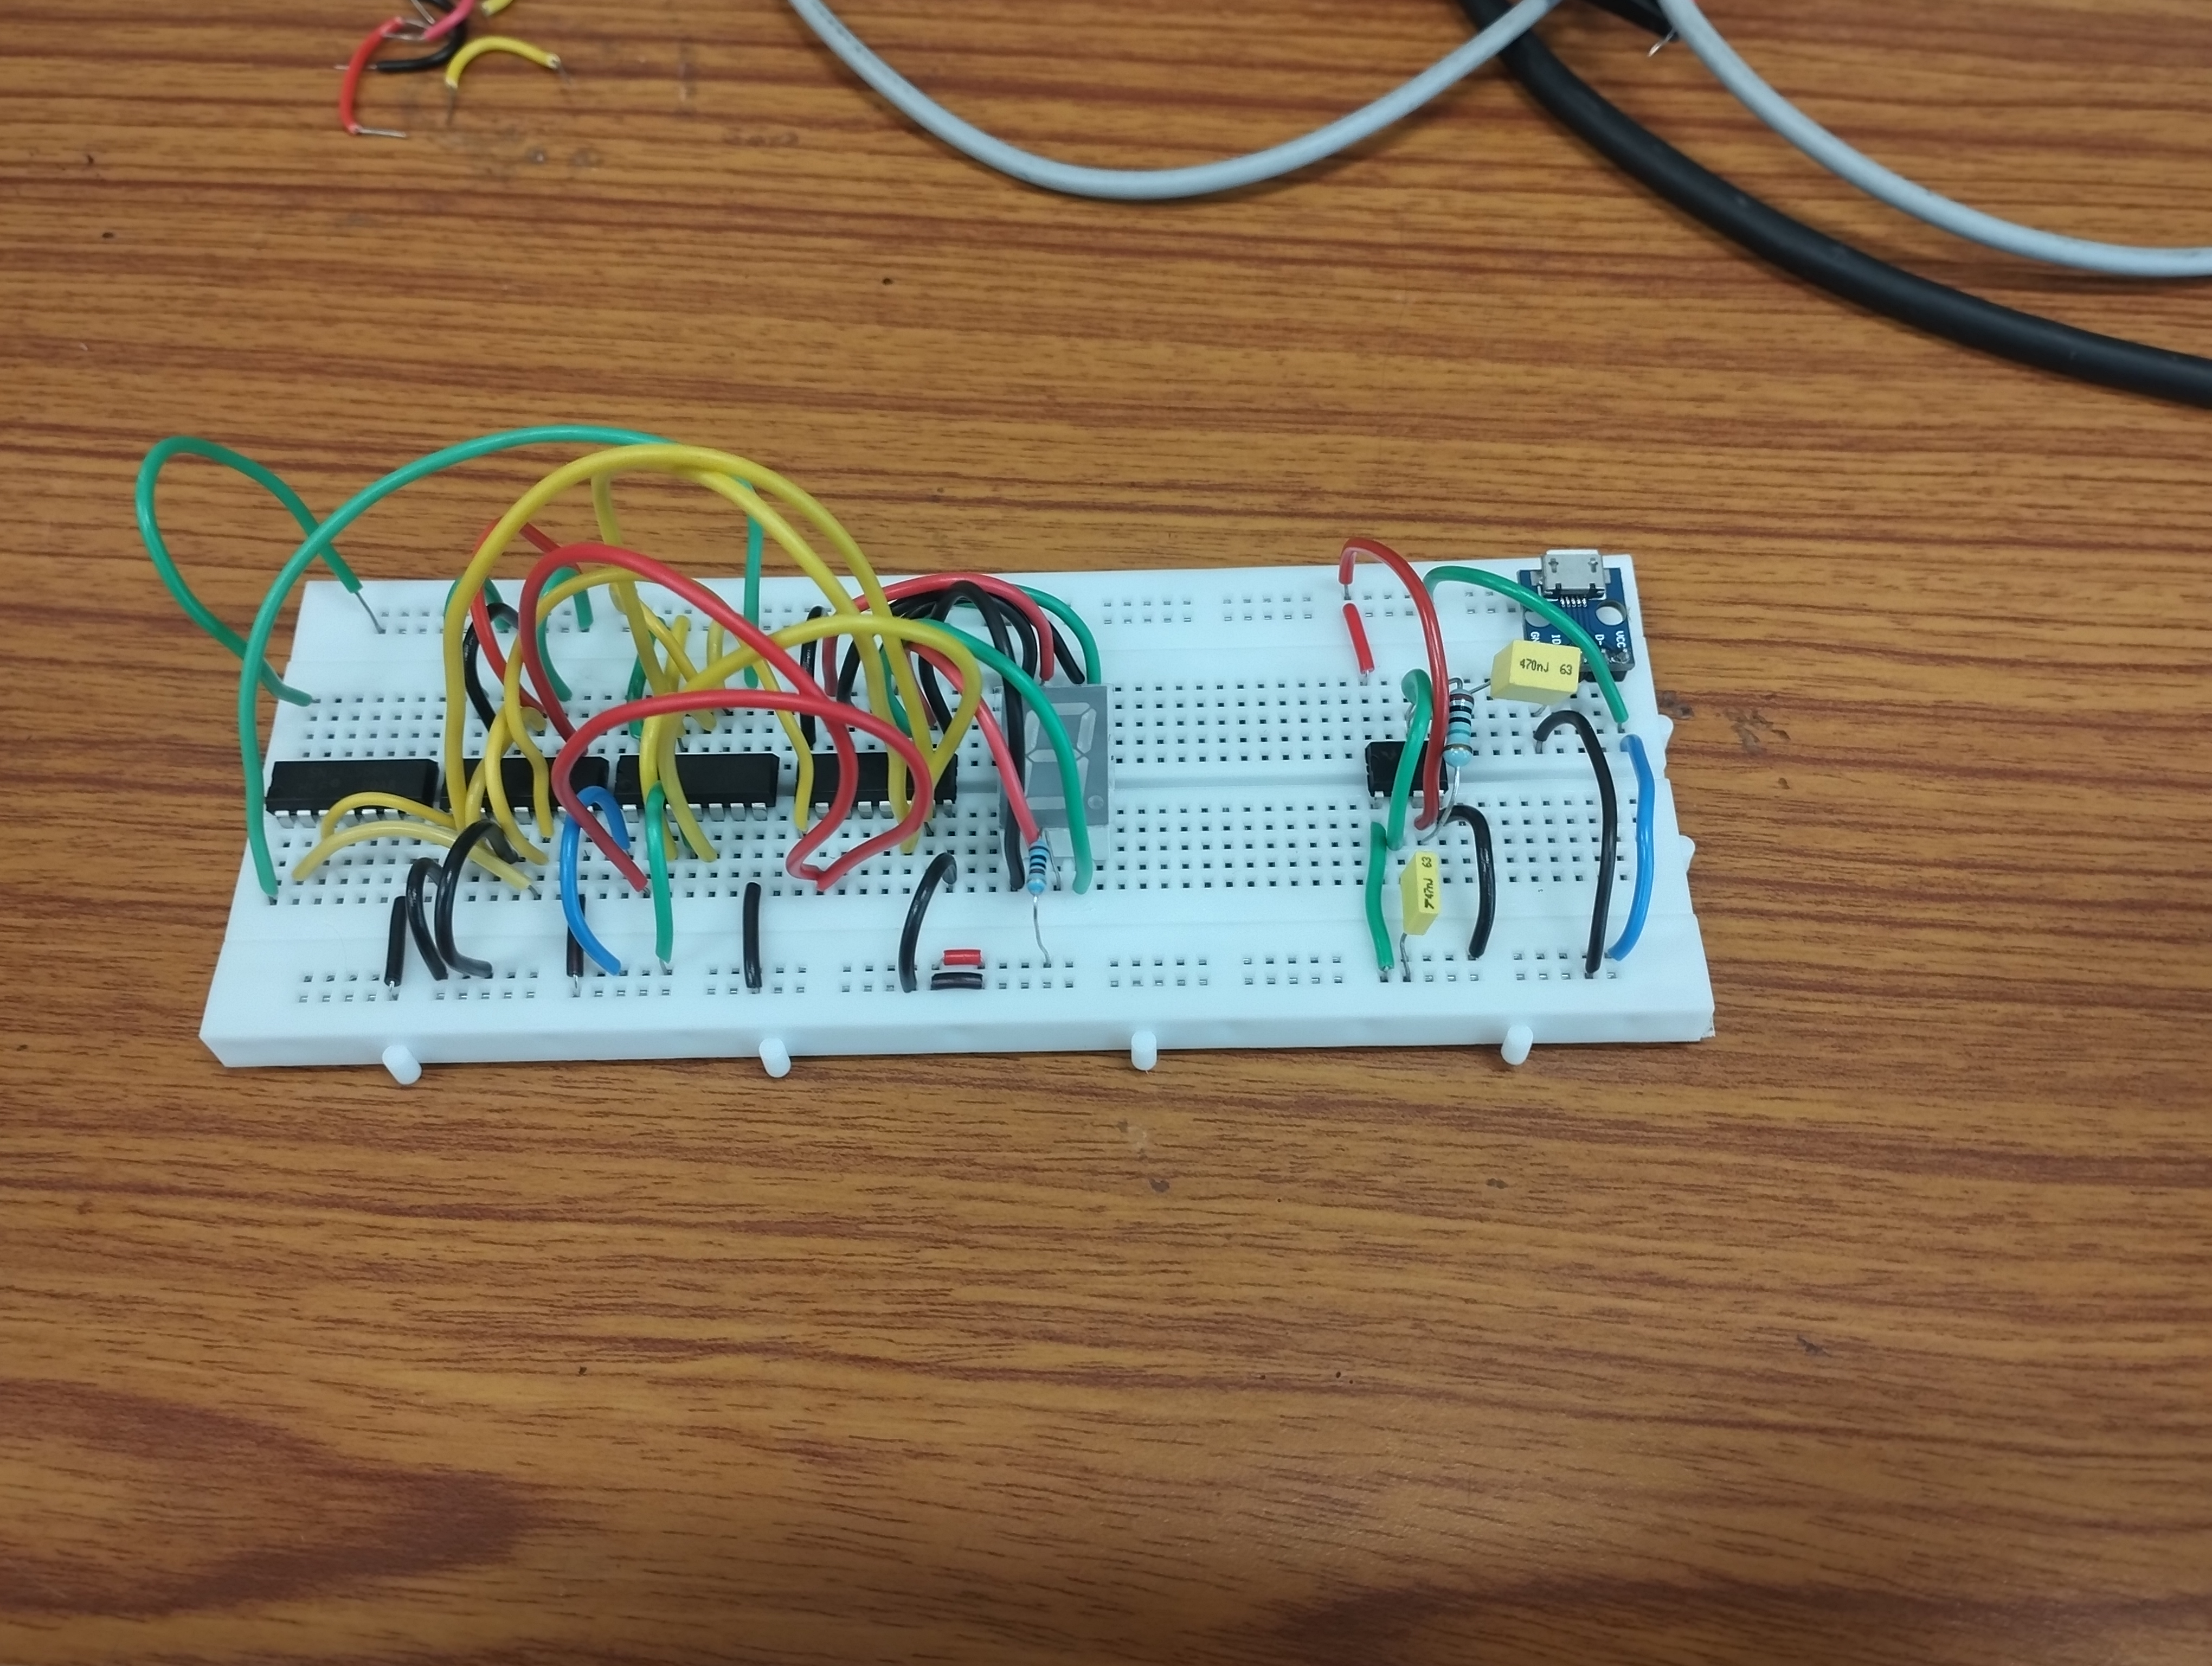
\includegraphics[width=0.7\linewidth]{figs/1.jpg}
	\caption{Image 1}
	\label{fig:view}
\end{figure}
\FloatBarrier

\begin{figure}[ht]
	\centering
	\includegraphics[width=0.7\linewidth]{figs/2.jpg}
	\caption{Image 2}
	\label{fig:view}
\end{figure}
\FloatBarrier

\begin{figure}[ht]
	\centering
	\includegraphics[width=0.7\linewidth]{figs/3.jpg}
	\caption{Image 3}
	\label{fig:view}
\end{figure}
\FloatBarrier

\section*{Block Diagram}

\begin{figure}[ht]
	\centering
	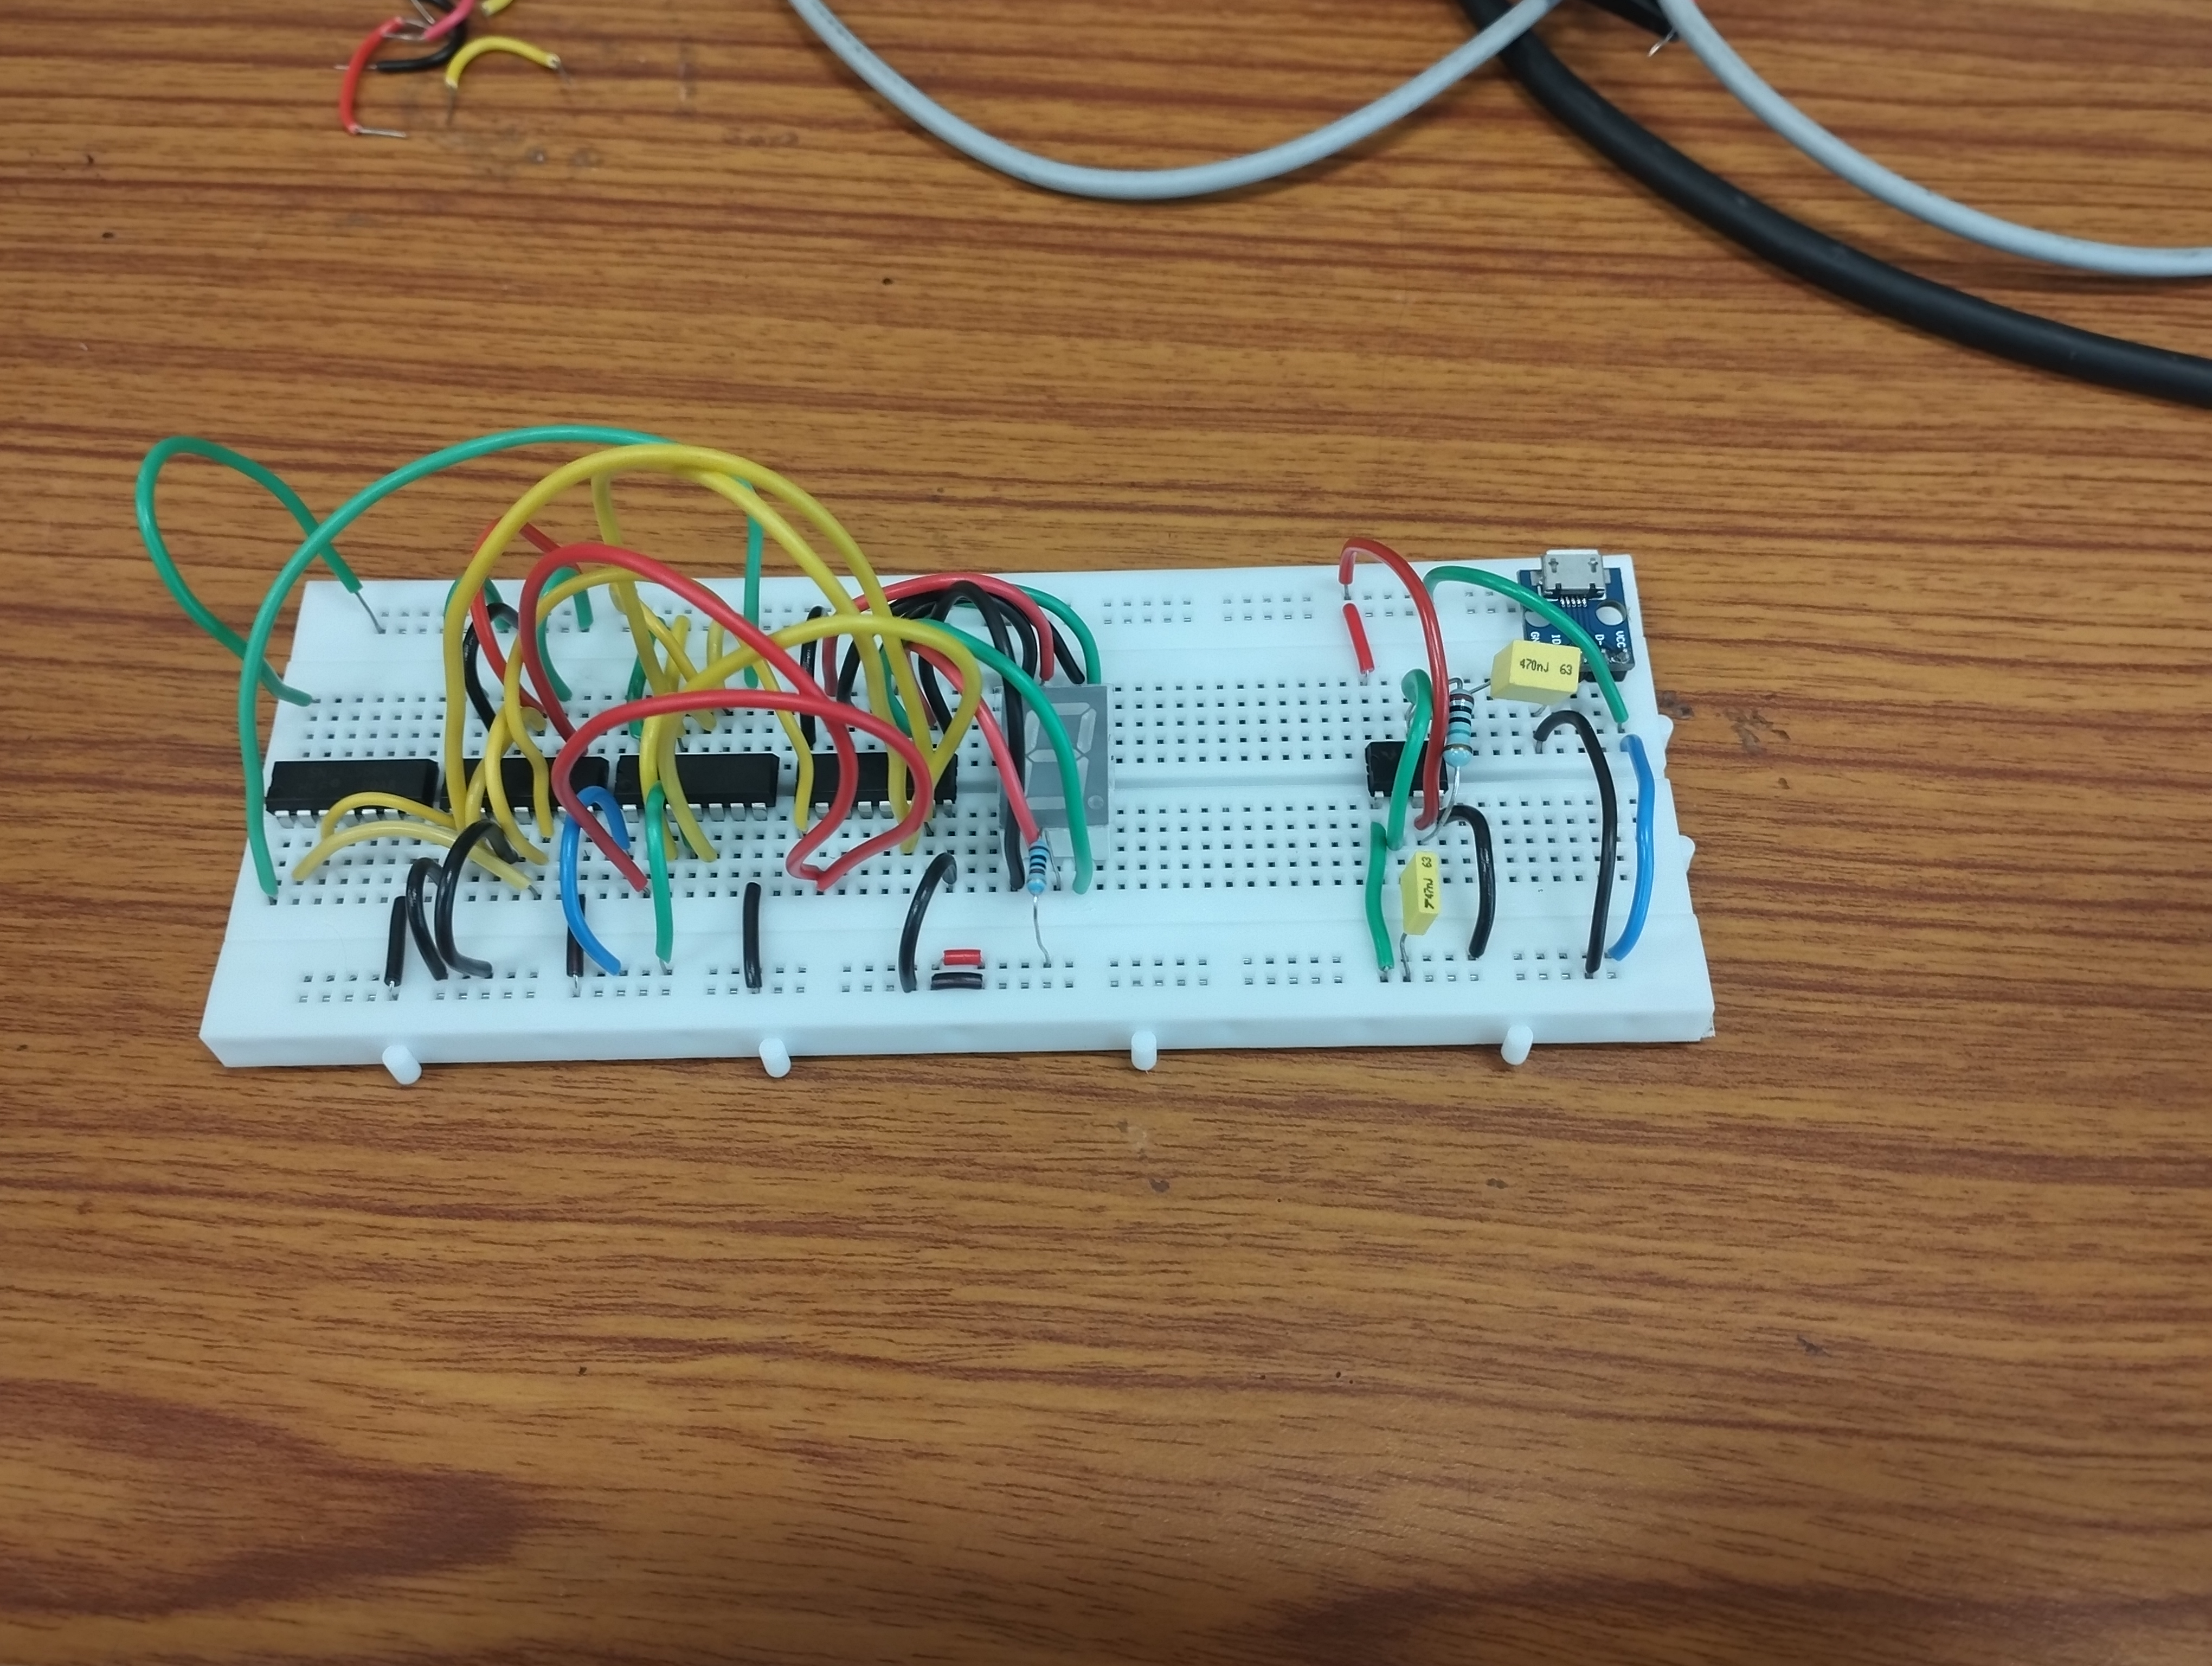
\includegraphics[width=0.7\linewidth]{figs/BlockDiagram.jpg}
	\caption{Block Diagram}
	\label{fig:view}
\end{figure}
\FloatBarrier


\end{document}
